\documentclass[tikz,crop]{standalone}
\usepackage{xcolor}
\usepackage{tikz}
\usetikzlibrary{calc,positioning,shadows,shadows.blur,matrix}

\def\slidersize{3.1cm}
\def\spacingslider{-0.3em}

\def\IosSevenSlider#1{
    \tikz[baseline=-0.1cm]{
        \coordinate (start) at (0,0);
        \coordinate (end) at (\slidersize,0);
        \coordinate (mark) at ($(start)!#1!(end)$);
        \useasboundingbox (start|- 0,-.25) rectangle (end|- 0, .25);
        \draw[line width=0.9mm, line cap=round, blue!50!cyan] 
             (start) -- (mark) edge[lightgray] (end);
        \node[fill=white, draw=lightgray, very thin,
            blur shadow={shadow xshift=0pt, shadow opacity=20, shadow yshift=-0.9mm,
                         shadow blur steps=6, shadow blur radius=0.3mm},
            circle, minimum size=0.25cm,yshift=3.4pt, inner sep=0pt] at (mark) {};
    }
}


\begin{document}
\setlength{\fboxsep}{0pt}
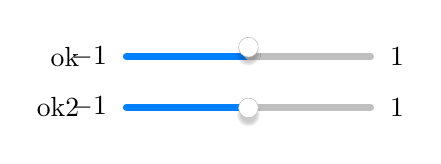
\begin{tikzpicture}

  \node (slider0) {\IosSevenSlider{0.5}};
  \node[left=0em of slider0.west, align=center] {$-1$};
  \node[right=0em of slider0.east, align=center] {$1$};
  \node[left=1em of slider0.west, align=right] {ok};



  \node[
    below=\spacingslider of slider0
  ] (slider1) {\IosSevenSlider{0.5}};
  \node[left=0em of slider1.west, align=center] {$-1$};
  \node[right=0em of slider1.east, align=center] {$1$};
  \node[left=1em of slider1.west, align=right] {ok2};

\end{tikzpicture}
\end{document}
